\documentclass[tikz,convert={outfile=\jobname.svg}]{standalone}
\usepackage{tikz}
\usetikzlibrary{automata, positioning, arrows.meta, bending} % 'positioning' is helpful for arranging nodes

\begin{document}
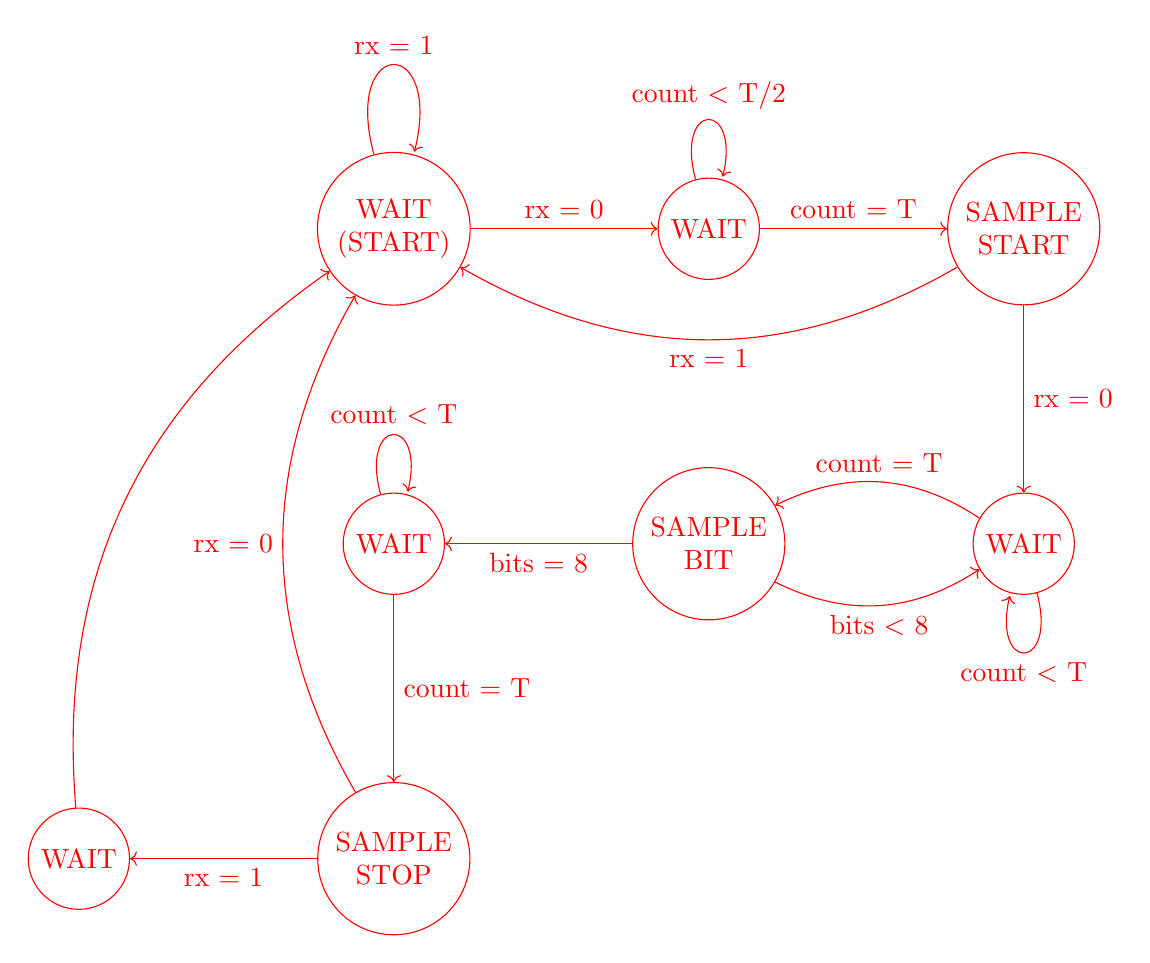
\begin{tikzpicture}[node distance=4cm, auto, state/.style={draw=red,shape=circle,text=red}, every node/.style={text=red}]

    % Define the states (nodes)
    \node[state, align=center] (s0) {WAIT\\(START)}; % Initial state 'q0'
    \node[state, right of=s0] (s1) {WAIT}; % Accepting state 'q1', positioned to the right of 'q0'
    \node[state, right of=s1, align=center] (s2) {
                    SAMPLE\\
                    START};
    \node[state, below of=s2] (s3) {WAIT};
    \node[state, left of=s3, align=center] (s4) {SAMPLE\\BIT};
    \node[state, left of=s4] (s5){WAIT};
    \node[state, below of=s5, align=center] (s6){SAMPLE\\STOP};
    \node[state, left of=s6] (s7){WAIT};
    % Define the transitions (edges)
    \path[->, draw=red] %[draw = red]
    (s0) edge node {rx = 0} (s1) % Transition from q0 to q1 labeled 'a'
    (s0) edge [loop above] node {rx = 1} (s0) % Transition from q1 to q0 labeled 'b'
    (s1) edge [loop above] node {count $<$ T/2} (s1) % Self-loop on q1 labeled 'a, b'
    (s1) edge node {count = T} (s2)
    (s2) edge node {rx = 0} (s3)
    (s2) edge [bend left] node {rx = 1} (s0)
    (s3) edge [loop below] node{count $<$ T}(s3)
    (s3) edge[bend right] node[above]{count = T} (s4)
    (s4) edge[bend right] node[below]{bits $<$ 8} (s3)
    (s4) edge node{bits = 8}(s5)
    (s5) edge[loop above] node{count $<$ T} (s5)
    (s5) edge node{count = T}(s6)
    (s6) edge[bend left] node{rx = 0} (s0)
    (s6) edge node{rx = 1} (s7)
    (s7) edge[bend left] (s0);
\end{tikzpicture}
\end{document}

